\documentclass[11pt,preprint]{elsarticle}

\usepackage{lmodern}
%%%% My spacing
\usepackage{setspace}
\setstretch{1.2}
\DeclareMathSizes{12}{14}{10}{10}

% Wrap around which gives all figures included the [H] command, or places it "here". This can be tedious to code in Rmarkdown.
\usepackage{float}
\let\origfigure\figure
\let\endorigfigure\endfigure
\renewenvironment{figure}[1][2] {
    \expandafter\origfigure\expandafter[H]
} {
    \endorigfigure
}

\let\origtable\table
\let\endorigtable\endtable
\renewenvironment{table}[1][2] {
    \expandafter\origtable\expandafter[H]
} {
    \endorigtable
}


\usepackage{ifxetex,ifluatex}
\usepackage{fixltx2e} % provides \textsubscript
\ifnum 0\ifxetex 1\fi\ifluatex 1\fi=0 % if pdftex
  \usepackage[T1]{fontenc}
  \usepackage[utf8]{inputenc}
\else % if luatex or xelatex
  \ifxetex
    \usepackage{mathspec}
    \usepackage{xltxtra,xunicode}
  \else
    \usepackage{fontspec}
  \fi
  \defaultfontfeatures{Mapping=tex-text,Scale=MatchLowercase}
  \newcommand{\euro}{€}
\fi

\usepackage{amssymb, amsmath, amsthm, amsfonts}

\def\bibsection{\section*{References}} %%% Make "References" appear before bibliography


\usepackage[numbers]{natbib}

\usepackage{longtable}
\usepackage[margin=2.3cm,bottom=2cm,top=2.5cm, includefoot]{geometry}
\usepackage{fancyhdr}
\usepackage[bottom, hang, flushmargin]{footmisc}
\usepackage{graphicx}
\numberwithin{equation}{section}
\numberwithin{figure}{section}
\numberwithin{table}{section}
\setlength{\parindent}{0cm}
\setlength{\parskip}{1.3ex plus 0.5ex minus 0.3ex}
\usepackage{textcomp}
\renewcommand{\headrulewidth}{0.2pt}
\renewcommand{\footrulewidth}{0.3pt}

\usepackage{array}
\newcolumntype{x}[1]{>{\centering\arraybackslash\hspace{0pt}}p{#1}}

%%%%  Remove the "preprint submitted to" part. Don't worry about this either, it just looks better without it:
\makeatletter
\def\ps@pprintTitle{%
  \let\@oddhead\@empty
  \let\@evenhead\@empty
  \let\@oddfoot\@empty
  \let\@evenfoot\@oddfoot
}
\makeatother

 \def\tightlist{} % This allows for subbullets!

\usepackage{hyperref}
\hypersetup{breaklinks=true,
            bookmarks=true,
            colorlinks=true,
            citecolor=blue,
            urlcolor=blue,
            linkcolor=blue,
            pdfborder={0 0 0}}


% The following packages allow huxtable to work:
\usepackage{siunitx}
\usepackage{multirow}
\usepackage{hhline}
\usepackage{calc}
\usepackage{tabularx}
\usepackage{booktabs}
\usepackage{caption}


\newenvironment{columns}[1][]{}{}

\newenvironment{column}[1]{\begin{minipage}{#1}\ignorespaces}{%
\end{minipage}
\ifhmode\unskip\fi
\aftergroup\useignorespacesandallpars}

\def\useignorespacesandallpars#1\ignorespaces\fi{%
#1\fi\ignorespacesandallpars}

\makeatletter
\def\ignorespacesandallpars{%
  \@ifnextchar\par
    {\expandafter\ignorespacesandallpars\@gobble}%
    {}%
}
\makeatother


% definitions for citeproc citations
\NewDocumentCommand\citeproctext{}{}
\NewDocumentCommand\citeproc{mm}{%
\href{\#cite.\detokenize{#1}}{#2}\nocite{#1}}

\makeatletter
% allow citations to break across lines
\let\@cite@ofmt\@firstofone
% avoid brackets around text for \cite:
\def\@biblabel#1{}
\def\@cite#1#2{{#1\if@tempswa , #2\fi}}
\makeatother
\newlength{\cslhangindent}
\setlength{\cslhangindent}{1.5em}
\newlength{\csllabelwidth}
\setlength{\csllabelwidth}{3em}
\newenvironment{CSLReferences}[2] % #1 hanging-indent, #2 entry-spacing
{\begin{list}{}{%
	\setlength{\itemindent}{0pt}
	\setlength{\leftmargin}{0pt}
	\setlength{\parsep}{0pt}
	% turn on hanging indent if param 1 is 1
	\ifodd #1
	\setlength{\leftmargin}{\cslhangindent}
	\setlength{\itemindent}{-1\cslhangindent}
	\fi
	% set entry spacing
	\setlength{\itemsep}{#2\baselineskip}}}
{\end{list}}

\usepackage{calc}
\newcommand{\CSLBlock}[1]{\hfill\break\parbox[t]{\linewidth}{\strut\ignorespaces#1\strut}}
\newcommand{\CSLLeftMargin}[1]{\parbox[t]{\csllabelwidth}{\strut#1\strut}}
\newcommand{\CSLRightInline}[1]{\parbox[t]{\linewidth - \csllabelwidth}{\strut#1\strut}}
\newcommand{\CSLIndent}[1]{\hspace{\cslhangindent}#1}


\urlstyle{same}  % don't use monospace font for urls
\setlength{\parindent}{0pt}
\setlength{\parskip}{6pt plus 2pt minus 1pt}
\setlength{\emergencystretch}{3em}  % prevent overfull lines
\setcounter{secnumdepth}{5}

%%% Use protect on footnotes to avoid problems with footnotes in titles
\let\rmarkdownfootnote\footnote%
\def\footnote{\protect\rmarkdownfootnote}
\IfFileExists{upquote.sty}{\usepackage{upquote}}{}

%%% Include extra packages specified by user

%%% Hard setting column skips for reports - this ensures greater consistency and control over the length settings in the document.
%% page layout
%% paragraphs
\setlength{\baselineskip}{12pt plus 0pt minus 0pt}
\setlength{\parskip}{12pt plus 0pt minus 0pt}
\setlength{\parindent}{0pt plus 0pt minus 0pt}
%% floats
\setlength{\floatsep}{12pt plus 0 pt minus 0pt}
\setlength{\textfloatsep}{20pt plus 0pt minus 0pt}
\setlength{\intextsep}{14pt plus 0pt minus 0pt}
\setlength{\dbltextfloatsep}{20pt plus 0pt minus 0pt}
\setlength{\dblfloatsep}{14pt plus 0pt minus 0pt}
%% maths
\setlength{\abovedisplayskip}{12pt plus 0pt minus 0pt}
\setlength{\belowdisplayskip}{12pt plus 0pt minus 0pt}
%% lists
\setlength{\topsep}{10pt plus 0pt minus 0pt}
\setlength{\partopsep}{3pt plus 0pt minus 0pt}
\setlength{\itemsep}{5pt plus 0pt minus 0pt}
\setlength{\labelsep}{8mm plus 0mm minus 0mm}
\setlength{\parsep}{\the\parskip}
\setlength{\listparindent}{\the\parindent}
%% verbatim
\setlength{\fboxsep}{5pt plus 0pt minus 0pt}



\begin{document}



\begin{frontmatter}  %

\title{Large, Mid and Small Caps: Risk and Return Profiles of the Local
Size Indexes}

% Set to FALSE if wanting to remove title (for submission)




\author[Add1]{Sihlelelwe Nzima}
\ead{}





\address[Add1]{Stellenbosch University, Stellenbosch, South Africa}


\begin{abstract}
\small{
This report compares the large, mid and small cap indexes on their
structure, risk and return. The three are very different bets on the
economy: large caps carry the market's global and resource exposure and,
since 2023, closely resemble the Capped SWIX, while mid and small caps
are concentrated in locally listed industrials, financials and property
and are, in effect, value bets. Large caps delivered the strongest
returns over 2015-2026. Small caps show the lowest index volatility and
the best Sharpe ratio, but only because their stocks rarely move
together; they suffered the deepest drawdown when they did. Mid caps
lagged over the decade but held up best in months of rand stress.
}
\end{abstract}

\vspace{1cm}


\begin{keyword}
\footnotesize{
Size indexes \sep Active share \sep Realised volatility
\sep Stratification \\
\vspace{0.3cm}
}
\footnotesize{
\textit{JEL classification} G11 \sep G12
}
\end{keyword}



\vspace{0.5cm}

\end{frontmatter}

\setcounter{footnote}{0}



%________________________
% Header and Footers
%%%%%%%%%%%%%%%%%%%%%%%%%%%%%%%%%
\pagestyle{fancy}
\chead{}
\rhead{}
\lfoot{}
\rfoot{\footnotesize Page \thepage}
\lhead{}
%\rfoot{\footnotesize Page \thepage } % "e.g. Page 2"
\cfoot{}

%\setlength\headheight{30pt}
%%%%%%%%%%%%%%%%%%%%%%%%%%%%%%%%%
%________________________

\headsep 35pt % So that header does not go over title




\section{\texorpdfstring{Introduction
\label{Introduction}}{Introduction }}\label{introduction}

Investors often treat the choice between large, mid and small cap
indexes as a choice about company size. This report argues that it is
mainly a choice about economic exposure and about the kind of risk being
taken. This report compares the three local size indexes on their
structure (sector exposure, concentration and active share against the
Capped SWIX), their risk (the realised volatility of their constituents,
diversification and GARCH volatility) and their returns (rolling
returns, risk-adjusted performance and a stratification of months by
rand and global stress).

\section{Data}\label{data}

Monthly constituent weights for the large, mid and small cap indexes and
the Capped SWIX are available from 2007, and daily index returns (J200,
J201, J202 and J433) from 2015. The structure analysis therefore covers
2007-2026 and the risk and return analysis 2015-2026. Weights are
rescaled to 100\% each month, and missing sectors are filled from other
months and from the daily constituent file; the remainder, almost
entirely older small caps, is labelled unclassified.

\section{Structure: what the size indexes
hold}\label{structure-what-the-size-indexes-hold}

Figure \ref{sectors} shows that the three indexes are very different
bets on the economy. Large caps were about half resources in 2007,
shifted towards industrials until around 2016, and are close to 40\%
resources again today. Mid caps began as an industrials index and have
become more balanced, while small caps are concentrated in industrials
and, increasingly, property (31\% of the index today). Moving down the
size spectrum therefore means swapping commodity exposure for locally
listed industrial, financial and property businesses, although, as
Section \ref{Beyond} shows, locally listed does not mean exposed to the
rand.

\begin{figure}[H]

{\centering 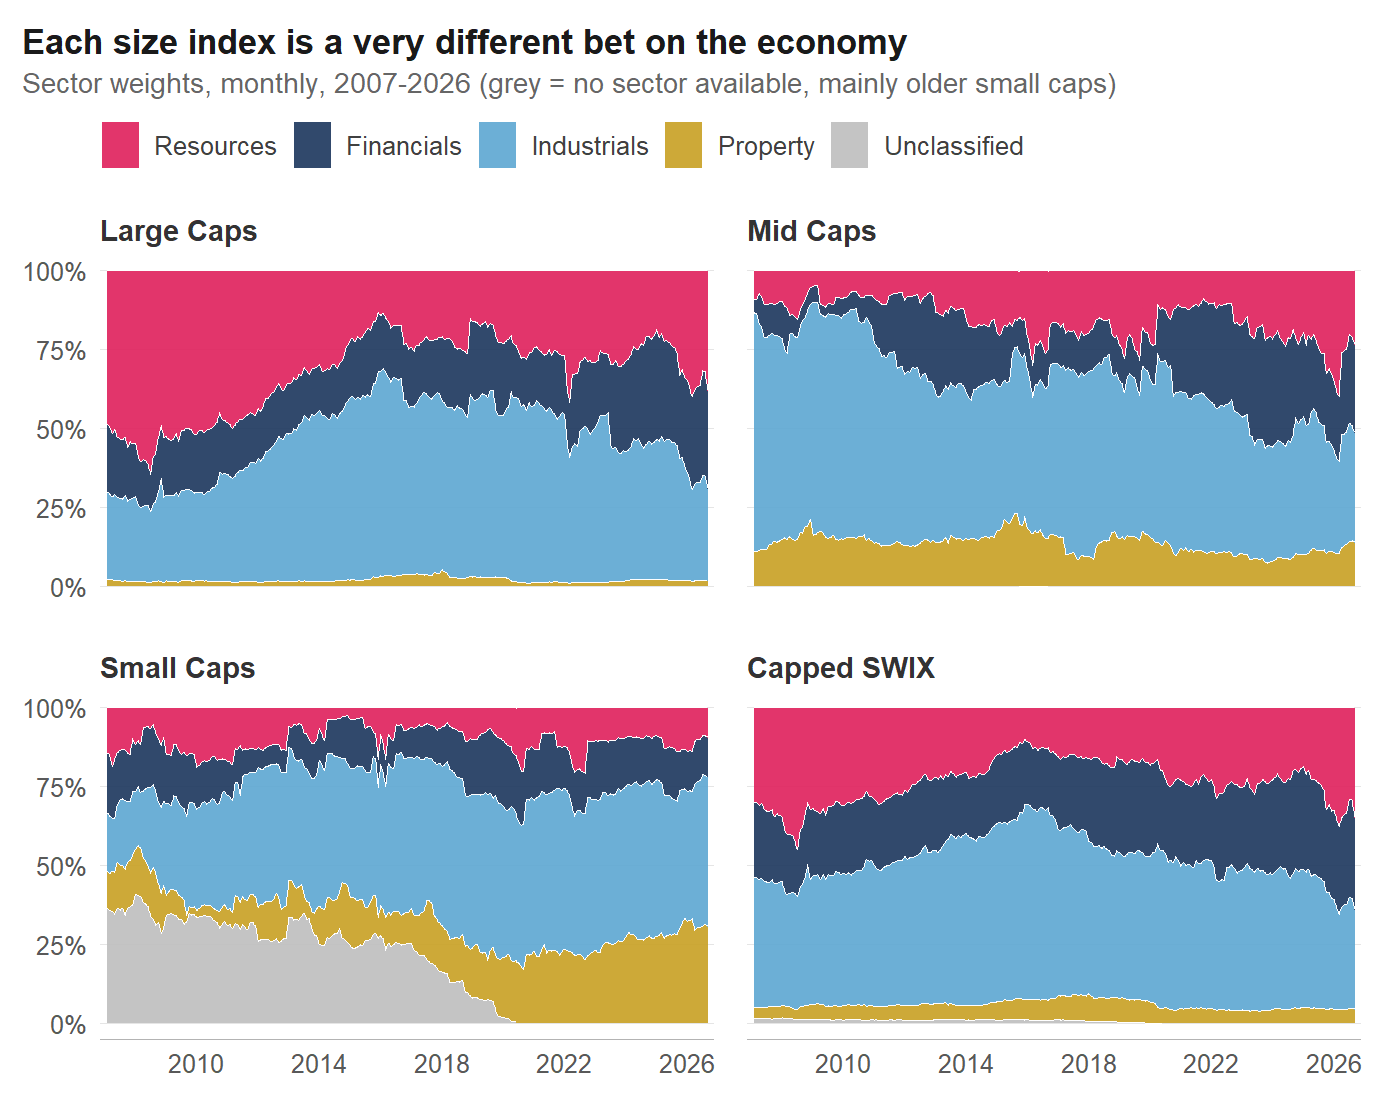
\includegraphics[width=1\linewidth]{Question2_files/figure-latex/sectors-1} 

}

\caption{Sector weights of the size indexes \label{sectors}}\label{fig:sectors}
\end{figure}

Figure \ref{concas} shows concentration with Lorenz curves, which plot
the cumulative share of stocks (smallest first) against the cumulative
share of index weight; the further a curve bows below the diagonal, the
more a few large stocks dominate, as summarised by the Gini coefficient.
Large caps were by far the most concentrated index in 2007 (Gini 0.55)
but have become much less so (0.44), while mid and small caps have moved
the other way (to 0.41 and 0.34). The biggest change came in June 2023,
when Richemont (about 22\% of the index) left the large cap holdings.
The right panel measures how different each index is from the broad
market by combining active share against the Capped SWIX,
\(\frac{1}{2}\sum_i |w_i^{index} - w_i^{SWIX}|\), with tracking error,
following the classification of Cremers and Petajisto (cut-offs of 60\%
active share and 8\% tracking error). Large caps have moved into the
closet-indexer corner, with an active share of 13\% and a tracking error
of only 2\% in 2026, so they are now close to a replica of the broad
market. Small caps are a consistently concentrated bet (active share of
about 95\% and tracking error of 9-19\% a year), while mid caps move
between the diversified and concentrated zones as their tracking error
rises in turbulent years.

\begin{figure}[H]

{\centering 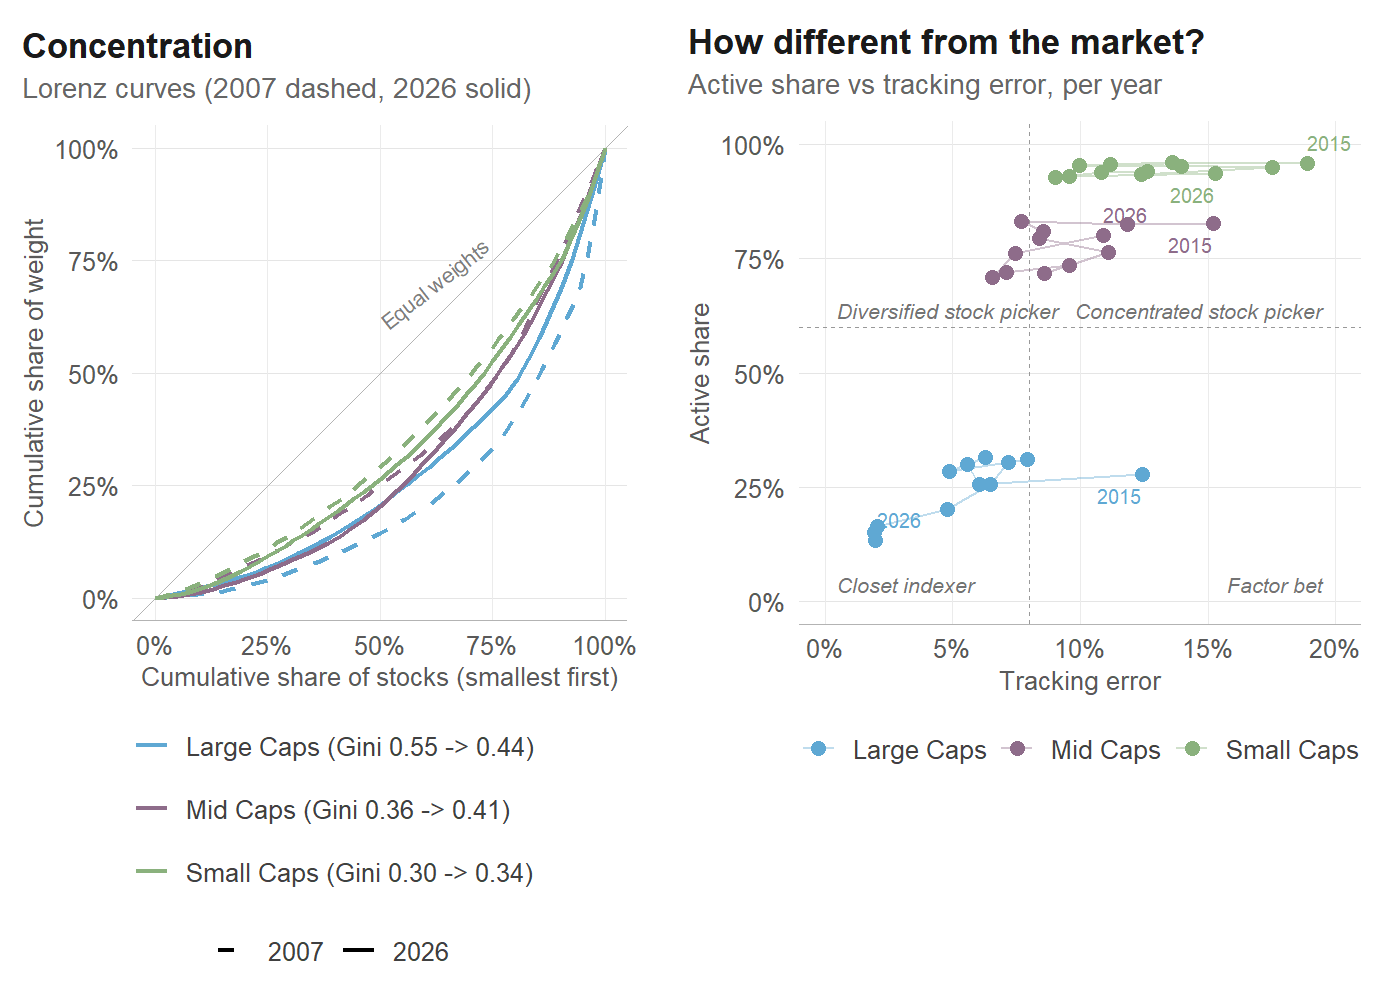
\includegraphics[width=1\linewidth]{Question2_files/figure-latex/concas-1} 

}

\caption{Lorenz curves (left) and active share vs tracking error against the Capped SWIX (right) \label{concas}}\label{fig:concas}
\end{figure}

\section{Risk}\label{risk}

Figure \ref{constvol} compares the realised volatility of the
constituents of each index over time. Outside crises the typical stock
is similarly volatile in all three indexes (a median of about 25-35\% a
year), but in stress small-cap stocks swing the most: during COVID-19
the median small-cap stock reached about 70\% volatility, against about
60\% for large and mid caps.

\begin{figure}[H]

{\centering 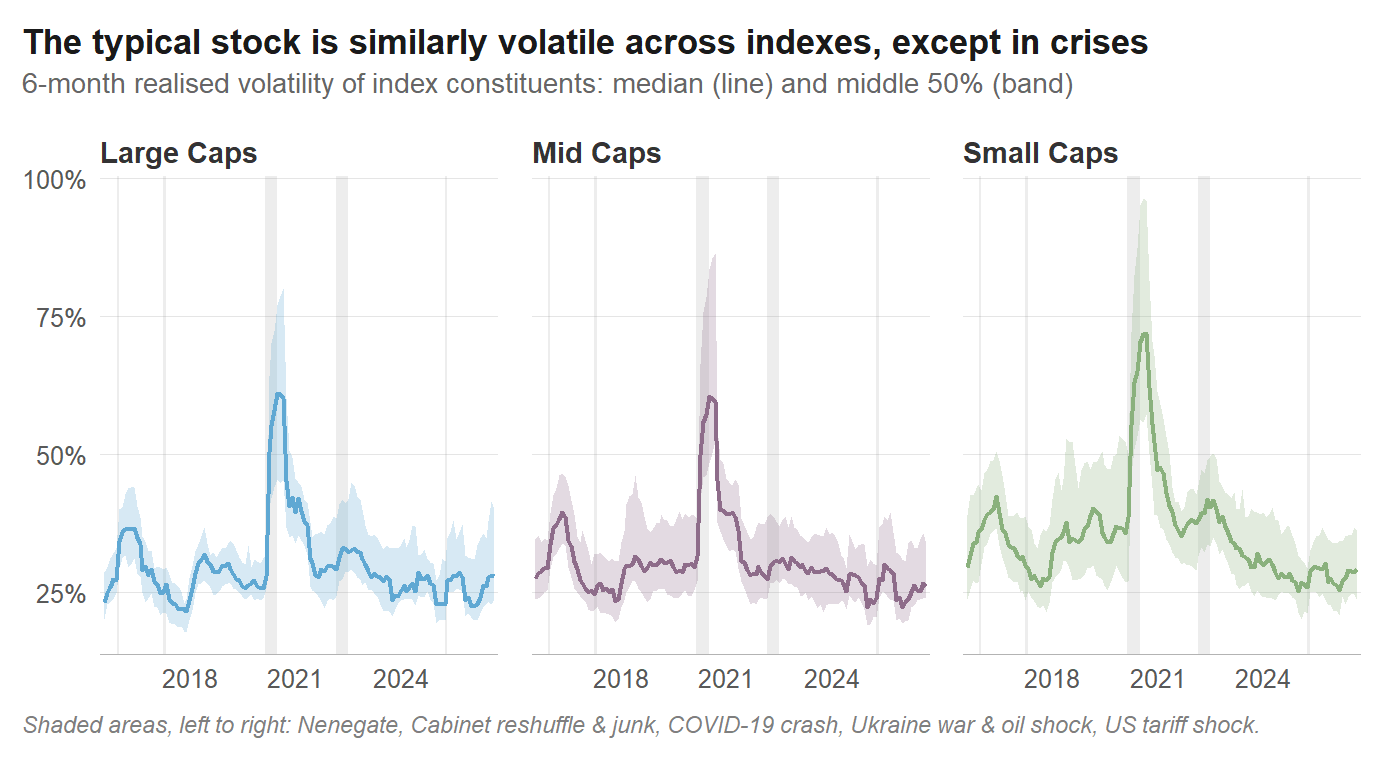
\includegraphics[width=1\linewidth]{Question2_files/figure-latex/constvol-1} 

}

\caption{Realised volatility of index constituents \label{constvol}}\label{fig:constvol}
\end{figure}

This raises a puzzle: small-cap stocks are individually at least as
volatile as large- and mid-cap stocks (and more so in crises), yet the
small cap \emph{index} is the least volatile of the three. Figure
\ref{div} resolves it by plotting, for every month, the weighted average
volatility of each index's stocks against the volatility of the index
itself. The large and mid cap months cluster around the line where the
index is half as volatile as its stocks; the small cap months sit close
to a quarter to a third, because small-cap stocks are driven by
company-specific news and many trade infrequently, so their moves
largely cancel out in the index. In crisis months the small cap points
move up towards the half-as-volatile line, as their stocks suddenly move
together, so their low index volatility understates their true risk.

\begin{figure}[H]

{\centering 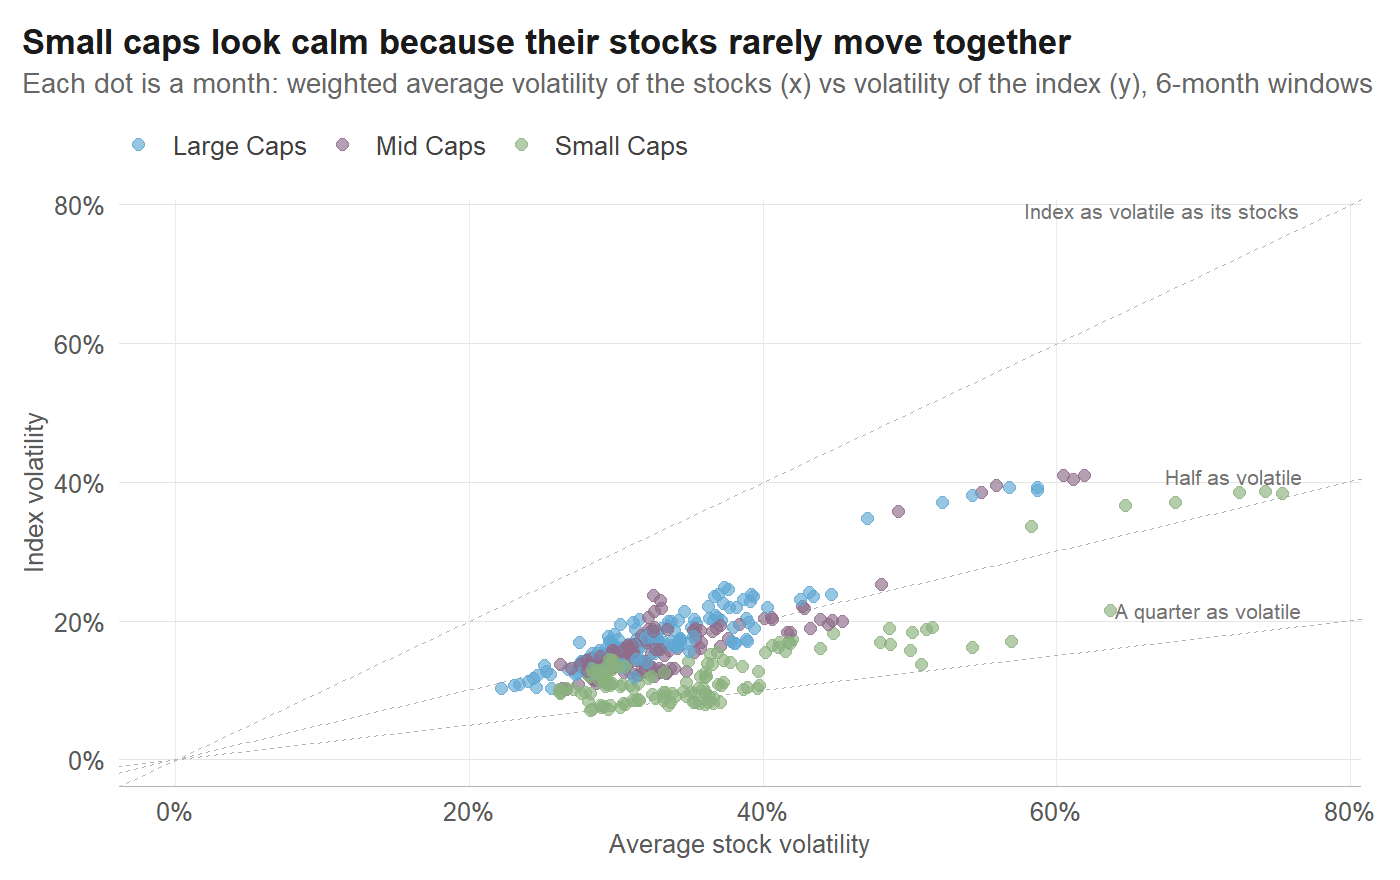
\includegraphics[width=1\linewidth]{Question2_files/figure-latex/div-1} 

}

\caption{Average stock volatility vs index volatility, monthly \label{div}}\label{fig:div}
\end{figure}

To see what kind of volatility each index faces, the same GJR-GARCH(1,1)
model as in Question 1 is fitted and used to draw news impact curves
(Figure \ref{newsimpact}): how much next-day volatility rises after a
daily shock of a given size and sign. After a 3\% fall, large-cap
volatility jumps from about 17\% to 25\% a year, but after a 3\% rise it
barely moves. Large caps therefore behave like the broad market, with
volatility triggered by global sell-offs (a leverage parameter of 0.14
and a symmetric parameter near zero). Small caps start from a much lower
base and react strongly in both directions, rising to about 21\% after a
3\% fall and 17\% after a 3\% rise, consistent with company-specific and
domestic drivers. Volatility shocks are short-lived in all three
indexes, with half-lives of 14-17 trading days.

\begin{figure}[H]

{\centering 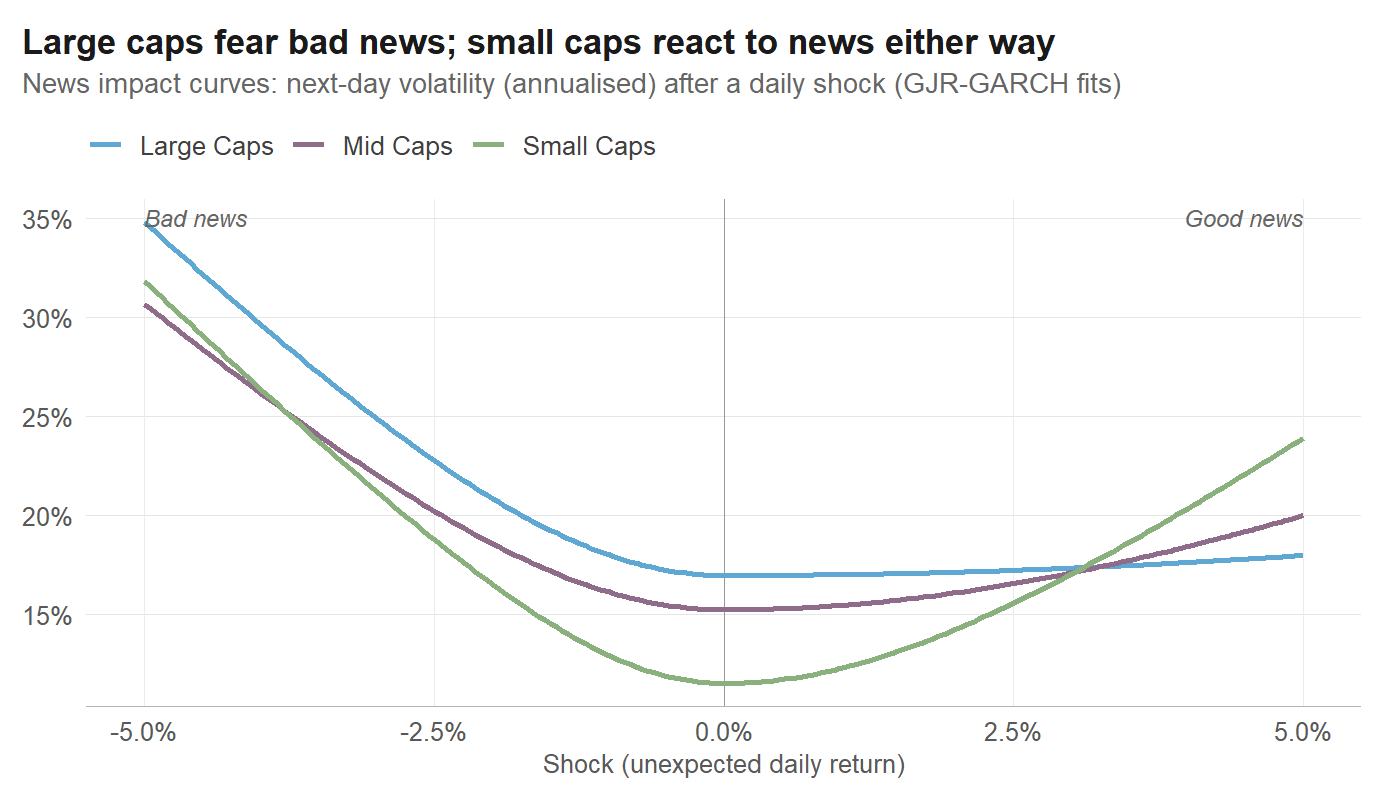
\includegraphics[width=1\linewidth]{Question2_files/figure-latex/newsimpact-1} 

}

\caption{News impact curves from GJR-GARCH(1,1) fits \label{newsimpact}}\label{fig:newsimpact}
\end{figure}

\section{Returns}\label{returns}

Rolling 1-year and 3-year returns relative to the Capped SWIX (Figure
\ref{rolling}, where each tile is one month) show how the ranking of the
indexes changes over time. Large caps beat the Capped SWIX in 88\% of
3-year windows, building most of their lead before 2022. Small caps are
the most cyclical: they fell furthest into the COVID-19 crash and then
led the market by up to 16\% a year during the recovery of 2021-2023.
Mid caps lagged the Capped SWIX in about two thirds of 3-year windows.

\begin{figure}[H]

{\centering 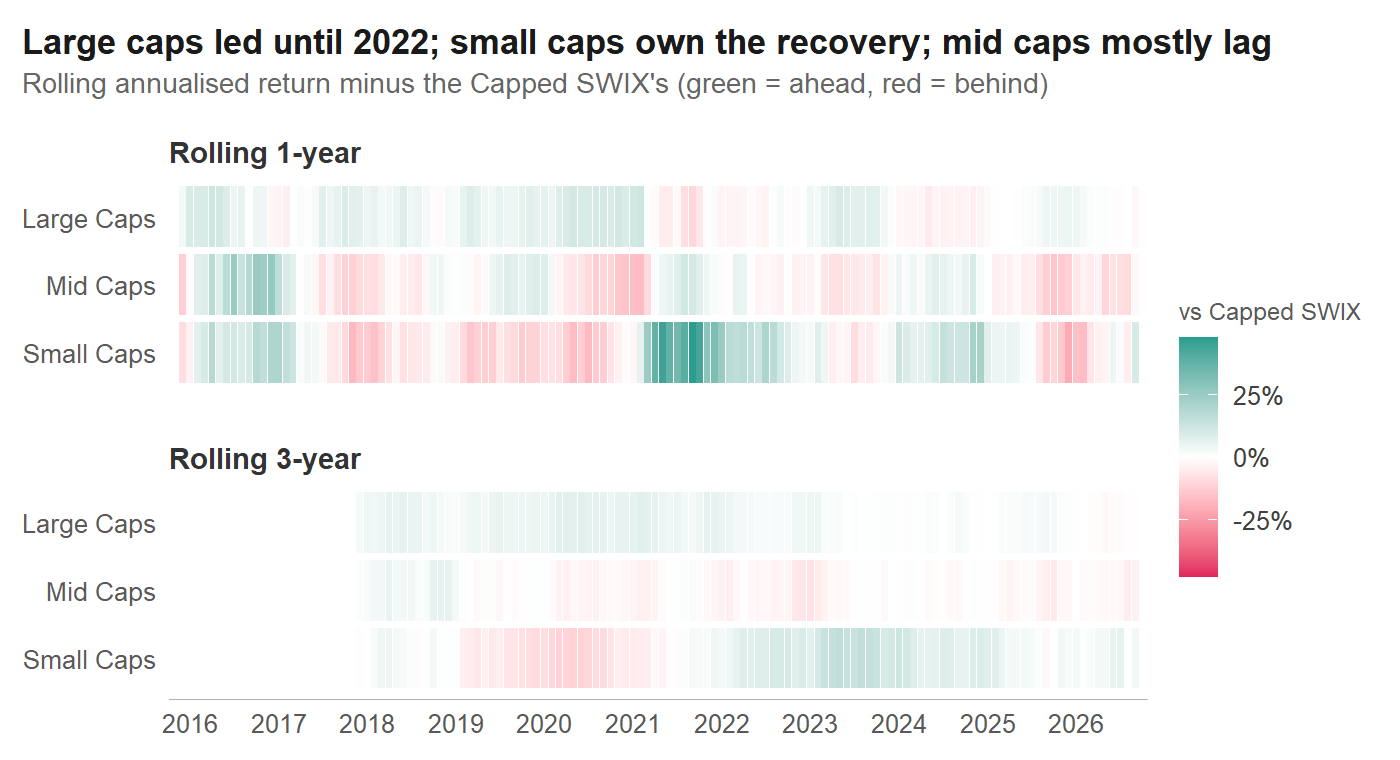
\includegraphics[width=1\linewidth]{Question2_files/figure-latex/rolling-1} 

}

\caption{Rolling returns relative to the Capped SWIX \label{rolling}}\label{fig:rolling}
\end{figure}

Over the full period (Figure \ref{riskreturn}) large caps returned about
11.0\% a year and small caps 10.3\%, both ahead of the Capped SWIX
(8.7\%), while mid caps returned 7.3\%. Small caps achieved the best
Sharpe ratio (0.25, using STeFI as the risk-free rate) thanks to their
low volatility, but also suffered by far the deepest drawdown (-51\%),
another sign that their measured volatility understates their risk. Mid
caps offered the weakest risk-return trade-off.

\begin{figure}[H]

{\centering 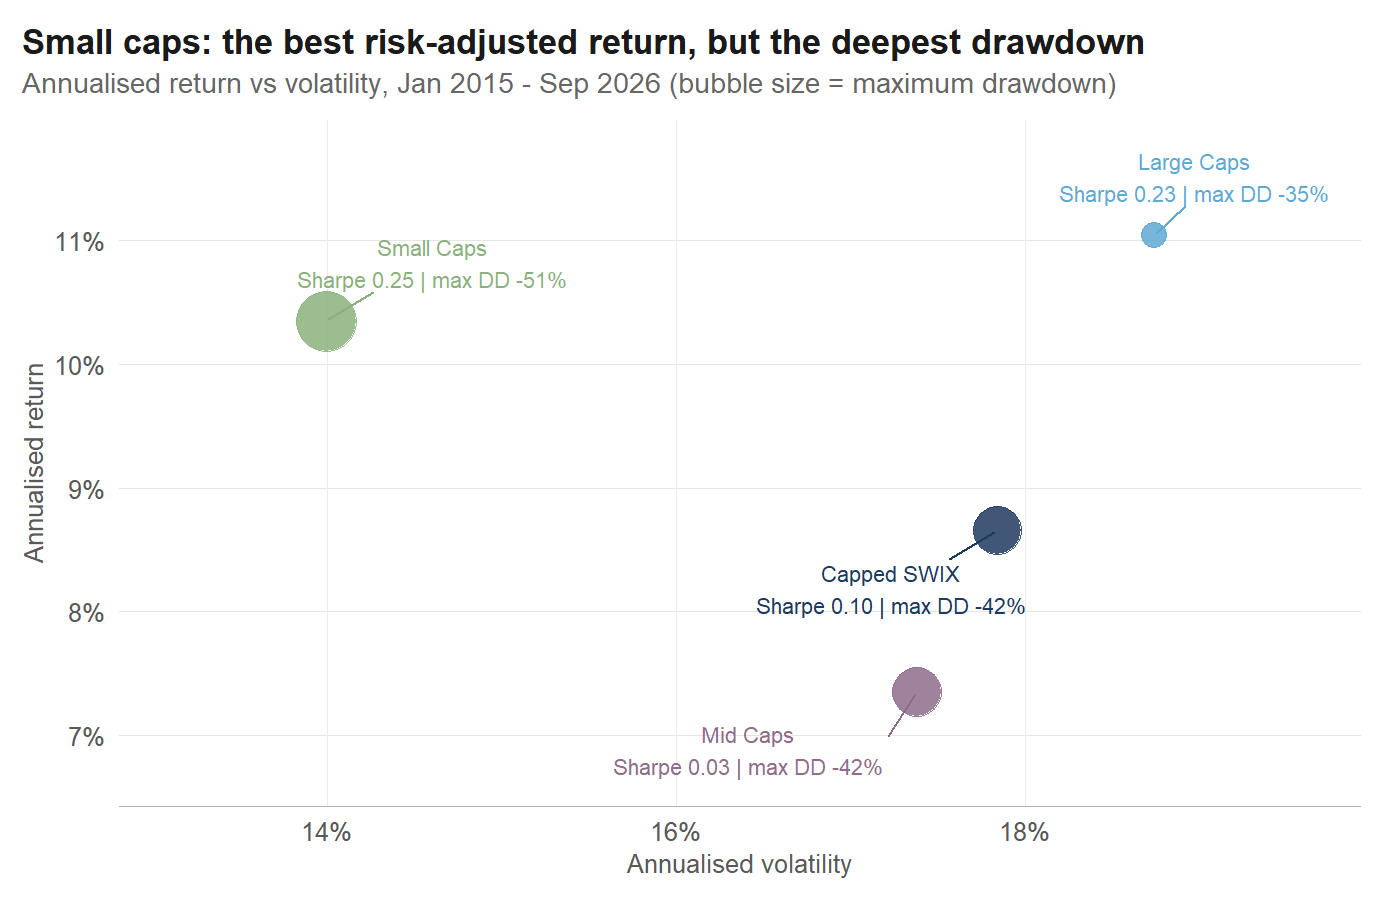
\includegraphics[width=1\linewidth]{Question2_files/figure-latex/riskreturn-1} 

}

\caption{Risk and return, 2015-2026 \label{riskreturn}}\label{fig:riskreturn}
\end{figure}

\section{Stratification: performance under
stress}\label{stratification-performance-under-stress}

Following the stratification approach of Practical 2, the analysis
identifies the months in the top and bottom 20\% of two stress measures,
rand volatility (SAVI) and the VIX, and compares each index in those
months with its full-sample behaviour, after winsorising daily returns
at the 1st and 99th percentiles. Figure \ref{strat} shows the full
spread of monthly returns in each regime. Rand stress is clearly bad for
local equities: in the calmest fifth of months for the rand the median
monthly return was 1.7-2.9\% for every index, but in the most stressed
fifth the Capped SWIX fell in 55\% of months, and large and small caps
did little better. Mid caps held up best, falling in only 38\% of
rand-stress months with a median return of +1.5\%. Global stress raises
volatility more than rand stress (by 30-40\% against 15-20\%), and most
for small caps relative to their normal level. Average returns are
higher in high-VIX months, but the much wider boxes show that these
months contain both the worst falls and the sharp rebounds that follow
sell-offs, such as in April-May 2020, so this reflects volatility rather
than genuine protection.

\begin{figure}[H]

{\centering 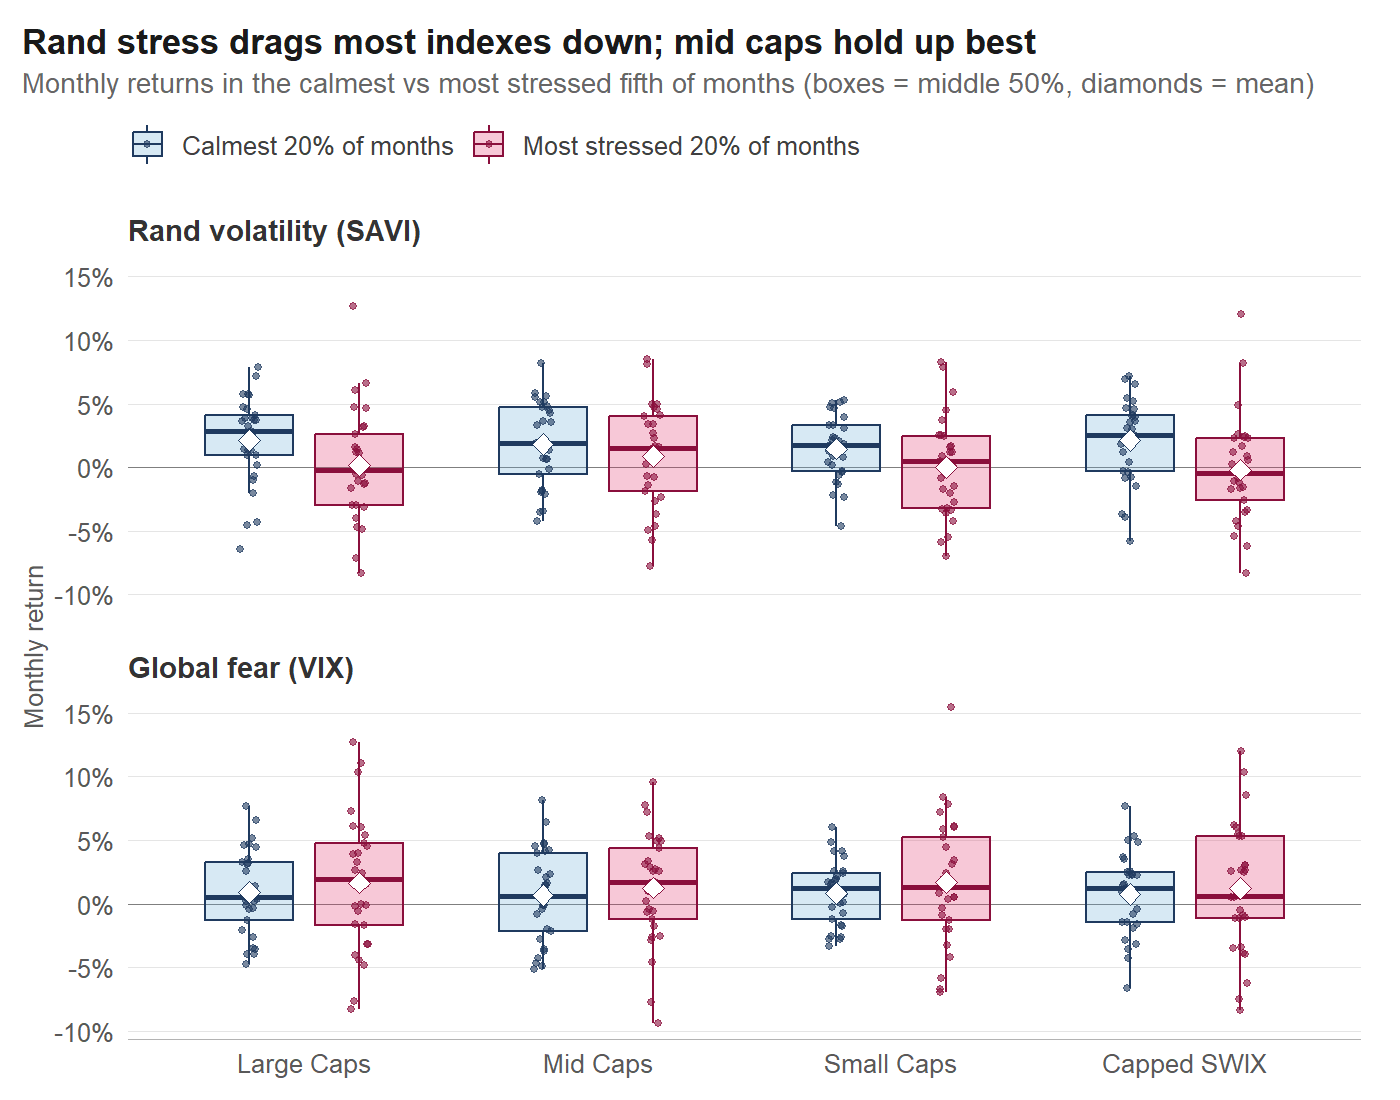
\includegraphics[width=1\linewidth]{Question2_files/figure-latex/strat-1} 

}

\caption{Monthly returns in calm vs stressed months, stratified by rand volatility and the VIX \label{strat}}\label{fig:strat}
\end{figure}

\section{\texorpdfstring{Beyond size: the hidden style and currency bets
\label{Beyond}}{Beyond size: the hidden style and currency bets }}\label{beyond-size-the-hidden-style-and-currency-bets}

The comparison so far raises a question the data can answer directly:
what is an investor really buying when choosing a size index? Applying
the same benchmark-relative factor scores and rand-hedge classification
used for SafeCore in Question 1 (Figure \ref{hidden}), the answer is
that size is largely a proxy for style. Large caps sit close to the
benchmark on every factor, mid caps are tilted towards value with weak
growth and negative momentum, and small caps are a deep-value bet
(+0.86) on stocks with poor recent momentum (-0.43). This helps explain
the return results: the mid and small cap indexes hold cheap,
out-of-favour stocks, which lagged over a decade led by the large caps,
while the strong small-cap recovery of 2021-2023 coincided with the
rebound in value stocks after COVID-19.

The currency profile overturns a common assumption. Small caps are not
the rand play they are often taken to be: they hold the most pure rand
hedges of any index (33\%, against 27\% for large caps) and the fewest
rand plays (10\%). Their largest rand hedges are property stocks such as
Vukile, Fortress and Resilient, consistent with the offshore property
portfolios several local REITs hold, alongside global businesses such as
Datatec and Bytes Technology. Mid caps have a currency mix close to the
broad market, so their resilience in rand-stress months is not explained
by currency hedges. Finally, the local size effect does not mirror the
global one: monthly small-minus-large returns are barely correlated with
the equivalent spread for MSCI World small and mid caps (a correlation
of 0.09). Unlike the volatility studied in Question 1, the relative
performance of the local size segments is driven by local factors.

\begin{figure}[H]

{\centering 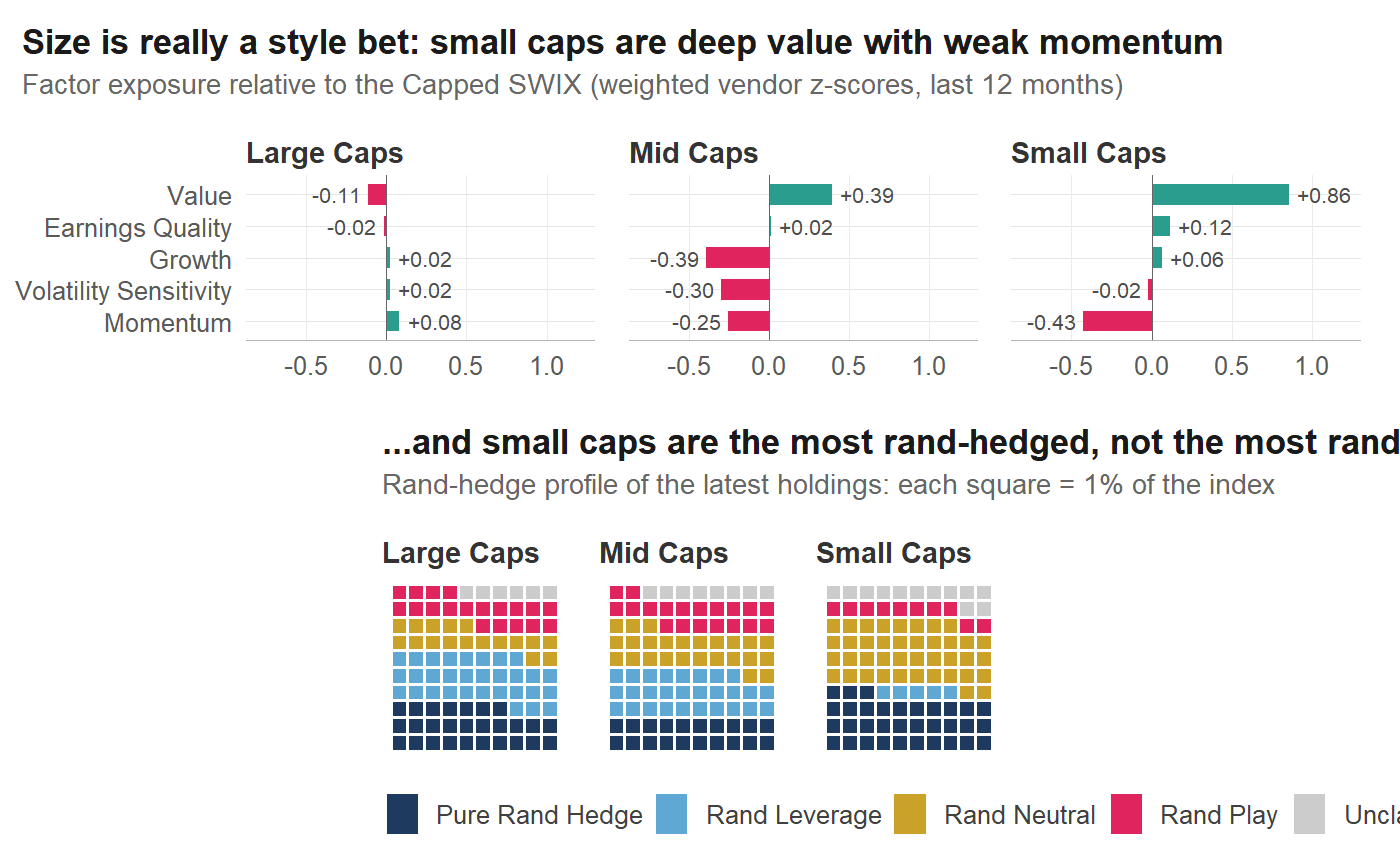
\includegraphics[width=1\linewidth]{Question2_files/figure-latex/hidden-1} 

}

\caption{Factor exposures relative to the Capped SWIX (left) and rand-hedge profiles (right) \label{hidden}}\label{fig:hidden}
\end{figure}

\section{\texorpdfstring{Conclusion
\label{Conclusion}}{Conclusion }}\label{conclusion}

The size indexes offer very different risk and return profiles. Large
caps delivered the strongest returns since 2015 and now closely resemble
the broad market, with volatility driven by global sell-offs. Small caps
look the safest on paper, with the lowest volatility and the best Sharpe
ratio, but this reflects stocks that rarely move together and trade
infrequently: in a crisis they move together and suffered the deepest
drawdown. Mid caps were the weakest segment over the decade, but held up
best in months of rand stress. For an investor, the choice is less about
company size than about exposure: large caps for global and resource
exposure, mid caps for a value-tilted exposure to local businesses, and
small caps for a deep-value bet that is, perhaps surprisingly, the most
rand-hedged segment of the market, bearing in mind that their smooth
returns hide significant crash risk.

\bibliography{Tex/ref}





\end{document}
